\documentclass[dvisvgm,tikz]{standalone}
\begin{document}
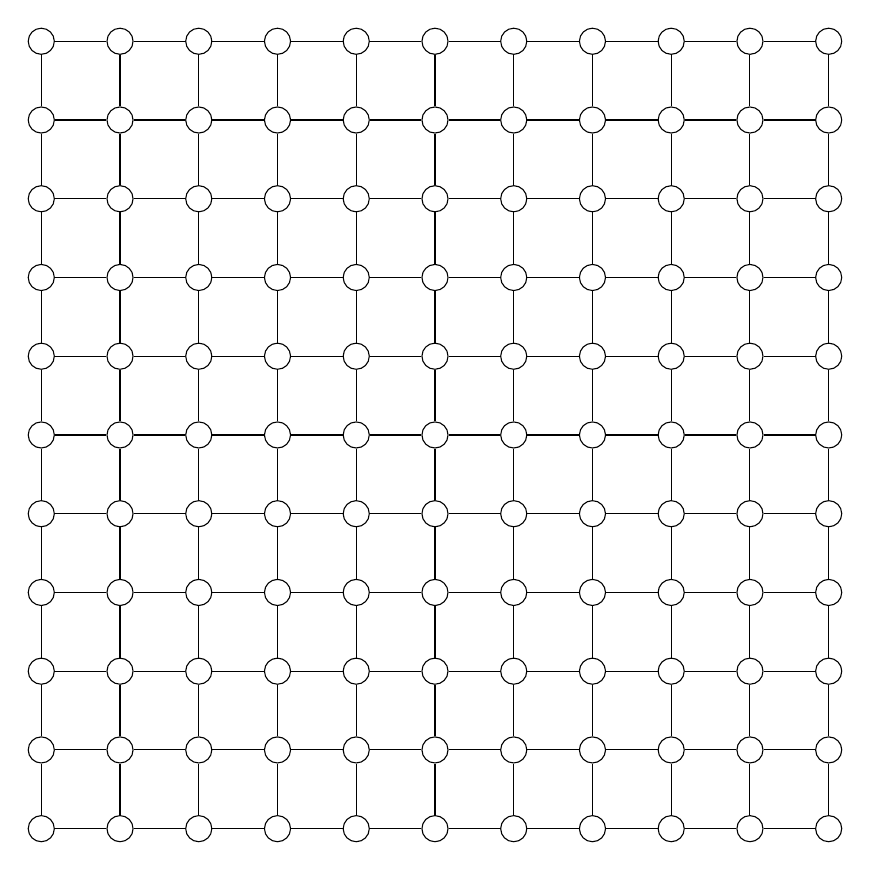
\begin{tikzpicture}

\foreach \x in {0,...,10}
  \foreach \y in {0,...,10} {
    \node[circle,draw] (\x\y) at (1.0+1.0*\x,1.0+1.0*\y) {};
  }

\foreach \x in {0,...,10}
  \foreach \y [count=\yi] in {0,...,9}
    \draw (\x\y)--(\x\yi) (\y\x)--(\yi\x);

\end{tikzpicture}
\end{document}
